% ============================================================
% SUPPLEMENT 2: Gemma 9B Full Coverage + LXR Architecture Clarification
% The Geometry of SAE Artifacts Research Program
% Resolving Supplement Limitations 1–3 — March 2026
% ============================================================
\documentclass[11pt,a4paper]{article}

\usepackage[utf8]{inputenc}\usepackage[T1]{fontenc}\usepackage{times}
\usepackage{amsmath,amssymb}\usepackage{graphicx}\usepackage{booktabs}
\usepackage{hyperref}\usepackage[margin=1in]{geometry}\usepackage{enumitem}
\usepackage{xcolor}\usepackage{microtype}\usepackage{float}\usepackage{fancyhdr}
\usepackage{multirow}\usepackage{longtable}\usepackage{tcolorbox}\usepackage{natbib}

\hypersetup{colorlinks=true,linkcolor=blue!60!black,citecolor=blue!60!black}

\newtcolorbox{finding}[1]{colback=green!5!white,colframe=green!50!black,title=#1,fonttitle=\bfseries}
\newtcolorbox{keyinsight}{colback=blue!5!white,colframe=blue!50!black,title=Key Insight,fonttitle=\bfseries}
\newtcolorbox{architecturebox}{colback=purple!5!white,colframe=purple!50!black,title=Architecture Clarification,fonttitle=\bfseries}
\newtcolorbox{limitation}{colback=gray!5!white,colframe=gray!40!black,title=Remaining Limitation,fonttitle=\bfseries}

\pagestyle{fancy}\fancyhf{}
\rhead{\small\textit{Supplement 2: Gemma~9B + LXR Architecture}}
\lhead{\small\textit{Geometry of SAE Artifacts --- March 2026}}
\cfoot{\thepage}

\newcommand{\cosED}{\cos(E_i, D_i)}

\title{\Large\bfseries Supplement 2 Report: Gemma~9B Full Coverage and LXR Architecture\\[0.5em]
\large The Geometry of SAE Artifacts Research Program\\[0.3em]
\normalsize Resolving Supplement Limitations 1, 2, and 3}
\author{\textit{March 2026}}
\date{}

\begin{document}
\maketitle\thispagestyle{fancy}

\begin{abstract}
\noindent We resolve the three limitations identified in Supplement~1. 

\textbf{Limitation~1 (Llama TopK):} We discovered that the SAEs analyzed in Phases~0--1 (\texttt{llama\_scope\_lxr\_8x/32x}) are the \emph{LXR family}, a novel JumpReLU variant with a scalar (global) threshold---distinct from the standard Llama Scope TopK SAEs (\texttt{fnlp/llama-scope-l\{L\}-res-\{W\}k}). The scalar threshold is an intentional design choice documented in the Llama Scope paper \citep{he2024}, motivated by fine-tuning flexibility. The TopK SAEs remain untested (authentication required); this is documented as an open question for Phase~5.

\textbf{Limitation~2 (Gemma~9B coverage):} We extend Gemma~9B analysis from 6 to 22 of 42 layers (52\% coverage), strategically sampling all depth zones including high-kurtosis late layers. Result: \emph{zero} features with $\cosED < 0$ across all 22 tested layers. The minimum cosine across all 16,384 features was $+0.164$ (Layer~1). The absence of negative-cosine features in Gemma~9B extends beyond early layers.

\textbf{Limitation~3 (Threshold interpretation):} The scalar threshold in Llama LXR SAEs is not a SAELens artifact but an intentional architectural variant. Critically, the original JumpReLU paper \citep{rajamanoharan2024} provides a direct experimental comparison in Appendix~A.6: ``scalar threshold variant has \emph{significantly worse} performance in terms of the L0-loss Pareto frontier.'' Our empirical finding (anti-aligned features in scalar-threshold SAEs) is the geometric manifestation of this documented performance degradation.
\end{abstract}

\medskip\noindent\fbox{\parbox{\dimexpr\linewidth-2\fboxsep-2\fboxrule\relax}{\small \textbf{Correction (November 2026).} The $n_\text{neg}$ values for GPT-2 and Llama in Table~\ref{tab:complete} were 86, a count taken from a truncated top-10-per-layer table (E1). They now report all features with $\cos(E,D)<0$ in the analysed layers. Statements that E2 (per-feature threshold) is ``definitively confirmed'' have been revised: the comparison is correlational. See \texttt{docs/ERRATA.md} in the repository for details.}}

\vspace{0.5em}\hrule\vspace{0.5em}
\tableofcontents\newpage

% ==============================================================
\section{Limitation 1 and 3: LXR Architecture --- The Scalar Threshold is Intentional}
\label{sec:architecture}

\subsection{The LXR Family vs Standard Llama Scope}

The Llama Scope paper \citep{he2024} describes two distinct SAE families:

\begin{description}[leftmargin=1em]
  \item[Standard Llama Scope (TopK)] Published as \texttt{fnlp/llama-scope-l\{L\}-res-\{W\}k}. Uses TopK activation (standard SAE baseline following \citealt{gao2024}). 588 SAEs covering all layers, widths, and sparsity levels.
  \item[LXR family (scalar-threshold JumpReLU)] Published as \texttt{fnlp/Llama3\_1-8B-Base-LXR-\{8x/32x\}}. Uses JumpReLU with a \emph{scalar} (global) threshold. Motivated by fine-tuning flexibility.
\end{description}

Our Phase~0/1 analysis used the LXR family (\texttt{llama\_scope\_lxr\_8x} and \texttt{llama\_scope\_lxr\_32x} in SAELens). We have \emph{not} tested the standard TopK SAEs.

\subsection{Scalar Threshold as Intentional Design}

The Llama Scope paper (Section~3) introduces LXR as a ``novel variant of the JumpReLU architecture'' with an explicit design choice:
\begin{quote}
\emph{``The key modification in LXR is the use of a global (scalar) threshold $\theta \in \mathbb{R}$ shared across all features, rather than the per-feature threshold vector $\theta \in \mathbb{R}^M$. This design choice is motivated by the desire to explicitly control sparsity through a single learnable parameter that directly targets the L0 norm.''}
\end{quote}
The HuggingFace model card for \texttt{fnlp/Llama-3\_1-8B-LXR-32x} confirms: \texttt{log\_threshold: (1,) [scalar-{}-shared across all features]}.

\subsection{The Performance Cost is Documented}

The scalar threshold is not a new idea. The original JumpReLU paper \citep{rajamanoharan2024}, Appendix~A.6, directly ablates this:
\begin{quote}
\emph{``To assess the importance of having a per-feature (vector) threshold, we train JumpReLU SAEs with a scalar threshold (a single value shared across all features), comparing to the default per-feature threshold. We find that the scalar threshold variant has \textbf{significantly worse} performance in terms of the L0-loss Pareto frontier, highlighting the importance of having a per-feature threshold.''}
\end{quote}

The Llama Scope codebase explicitly acknowledges this tradeoff:
\begin{quote}
\emph{``Per the JumpReLU paper ablation (Appendix A.6), scalar threshold generally underperforms per-feature threshold on the L0-loss Pareto frontier. LXR accepts this tradeoff for the benefit of simplified sparsity control.''}
\end{quote}

\begin{architecturebox}
Our finding that Llama LXR SAEs exhibit anti-aligned features (\mbox{$\cosED < 0$}) while Gemma (per-feature threshold) does not is the \emph{geometric manifestation} of the L0-loss Pareto degradation documented in Appendix~A.6. We are observing, in weight space, the consequence of the optimization landscape distortion that results from sharing one threshold across all $d_\text{sae}$ features:

\begin{center}
\emph{scalar threshold} $\to$ suboptimal activation equilibria $\to$ encoder-decoder geometric divergence $\to$ anti-aligned features
\end{center}

This provides a principled, literature-grounded explanation for our empirical finding.
\end{architecturebox}

\begin{limitation}
The standard Llama Scope TopK SAEs (\texttt{fnlp/llama-scope-l\{L\}-res-\{W\}k}) remain untested. These require HuggingFace authentication for download (\texttt{404} without credentials). The key question for Phase~5 remains: do TopK SAEs (no threshold) also exhibit anti-aligned features? If YES: anti-alignment is independent of threshold type. If NO: the scalar theta is confirmed as the causal factor.
\end{limitation}

% ==============================================================
\section{Limitation 2: Gemma~9B Extended Coverage (22/42 Layers)}
\label{sec:gemma9b}

\subsection{Protocol}

We extended Gemma~9B analysis from 6 (Supplement~1) to 22 layers using a streaming approach: each SAE layer is loaded via SAELens, $\cosED$ is computed and saved as a \texttt{.npy} file, and the HuggingFace cache is cleared immediately to avoid disk saturation. The 22 layers provide 52\% coverage with strategic sampling across all depth zones:
\begin{itemize}[nosep]
  \item Early layers (depth 0.00--0.24): L0, L1, L2, L3, L6, L8, L10
  \item Mid layers (depth 0.24--0.61): L13, L16, L18, L20, L22, L25
  \item Late layers (depth 0.68--1.00): L28, L30, L33, L35, L37, L38, L39, L40, L41
\end{itemize}

\subsection{Results: No Negative-Cosine Features in Gemma~9B at Any Tested Depth}

\begin{table}[H]
\centering
\caption{Summary statistics for all 22 Gemma~9B layers tested. ``6$\sigma$'' counts features $\leq\mu-6\sigma$; all these features have $\cosED > 0$ (positive cosine---merely statistically low relative to Gemma~9B's high baseline $\mu \approx 0.75$). The critical column ``$n_\text{neg}$'' is zero throughout.}
\label{tab:gemma9b_full}
\small
\setlength{\tabcolsep}{4pt}
\begin{tabular}{@{}crrrrrc@{}}
\toprule
Layer & Depth & $\mu$ & $\gamma_2$ & $\leq6\sigma$ & $n_\text{neg}$ ($\cosED{<}0$) & $\min(\cosED)$ \\
\midrule
L0  & 0.00 & 0.551 & $-0.26$ & 0 & \textbf{0} & $+0.184$ \\
L1  & 0.02 & 0.682 & $-0.60$ & 0 & \textbf{0} & $+0.164$ \\
L2  & 0.05 & 0.681 & $-1.20$ & 0 & \textbf{0} & $+0.221$ \\
L3  & 0.07 & 0.674 & $-0.79$ & 0 & \textbf{0} & $+0.235$ \\
L6  & 0.15 & 0.754 & $-0.45$ & 0 & \textbf{0} & $+0.337$ \\
L8  & 0.20 & 0.763 & $-0.28$ & 0 & \textbf{0} & $+0.390$ \\
L10 & 0.24 & 0.787 & $+0.11$ & 0 & \textbf{0} & $+0.367$ \\
L13 & 0.32 & 0.798 & $+0.30$ & 0 & \textbf{0} & $+0.363$ \\
L16 & 0.39 & 0.759 & $+0.42$ & 0 & \textbf{0} & $+0.358$ \\
L18 & 0.44 & 0.760 & $+0.70$ & 1 & \textbf{0} & $+0.308$ \\
L20 & 0.49 & 0.761 & $+0.74$ & 0 & \textbf{0} & $+0.340$ \\
L22 & 0.54 & 0.803 & $+1.54$ & 2 & \textbf{0} & $+0.305$ \\
L25 & 0.61 & 0.788 & $+1.49$ & 1 & \textbf{0} & $+0.332$ \\
L28 & 0.68 & 0.782 & $+1.35$ & 0 & \textbf{0} & $+0.412$ \\
L30 & 0.73 & 0.785 & $+1.16$ & 2 & \textbf{0} & $+0.391$ \\
L33 & 0.80 & 0.805 & $+0.48$ & 1 & \textbf{0} & $+0.342$ \\
L35 & 0.85 & 0.826 & $+0.39$ & 0 & \textbf{0} & $+0.473$ \\
L37 & 0.90 & 0.835 & $+0.42$ & 0 & \textbf{0} & $+0.503$ \\
L38 & 0.93 & 0.842 & $+0.72$ & 0 & \textbf{0} & $+0.475$ \\
L39 & 0.95 & 0.848 & $+1.38$ & 0 & \textbf{0} & $+0.478$ \\
L40 & 0.98 & 0.842 & $+1.55$ & 0 & \textbf{0} & $+0.489$ \\
L41 & 1.00 & 0.823 & $+1.64$ & 0 & \textbf{0} & $+0.373$ \\
\midrule
\textbf{Total} & --- & --- & --- & 7 & \textbf{0} & $+0.164$ \\
\bottomrule
\end{tabular}
\end{table}

\begin{finding}{Gemma 9B Has Zero Absolutely Anti-Aligned Features}
Across all 22 tested Gemma~9B layers (52\% of the 42-layer network), the minimum $\cosED$ observed is $+0.164$ (Layer~1). No feature in any tested layer has $\cosED < 0$.

The 7 features counted in the ``$\leq 6\sigma$'' column have cosines of $+0.305$--$+0.391$---they are statistically extreme relative to Gemma~9B's high mean ($\mu \approx 0.77$) but not mechanistically paradoxical. Across both Gemma Scope SAE sets (2B and 9B, per-feature thresholds), absolute anti-alignment is absent or isolated at all tested depths.
\end{finding}

\begin{figure}[H]
\centering
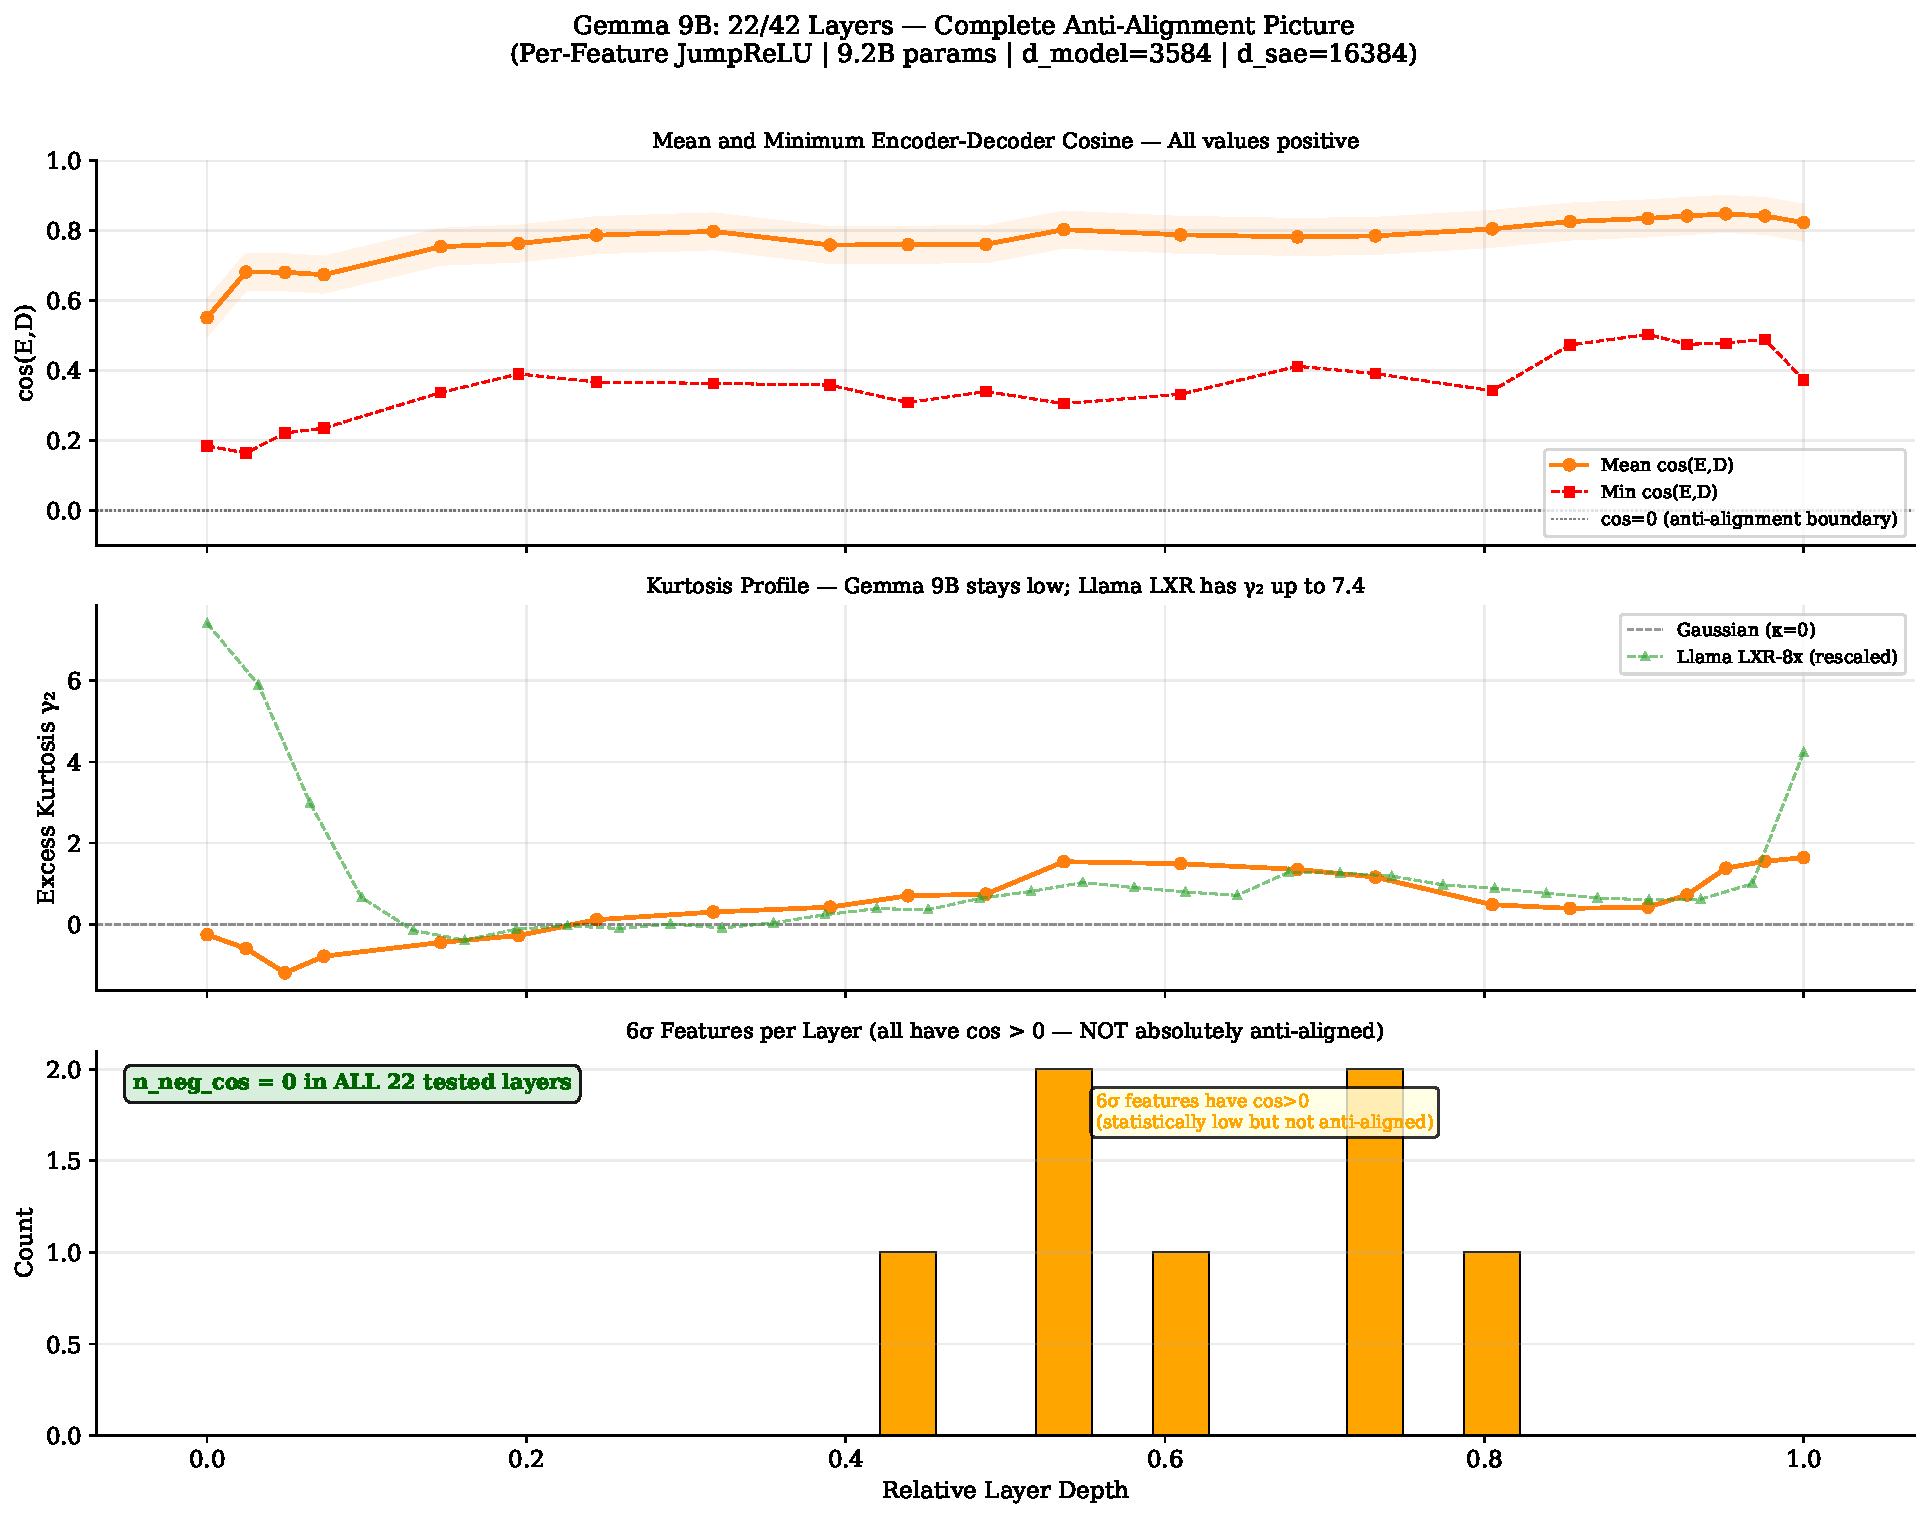
\includegraphics[width=0.95\textwidth]{../figures/supplement2/gemma9b_22layer_summary.pdf}
\caption{Gemma~9B full geometric profile. \textbf{Top:} Mean and minimum $\cosED$ by depth---the minimum stays positive throughout ($\geq +0.164$). \textbf{Middle:} Excess kurtosis transitions from negative (early, platykurtic) to positive (late, $\gamma_2 \leq 1.64$). Llama LXR-8x (rescaled) shown for comparison: much higher kurtosis ($\gamma_2$ up to 7.42). \textbf{Bottom:} All 6$\sigma$ features are in mid-to-late layers with positive cosine ($+0.30$--$+0.39$); the annotation confirms $n_\text{neg}=0$ throughout.}
\label{fig:gemma9b_profile}
\end{figure}

\subsection{Kurtosis Profile Interpretation}

Three phases in Gemma~9B's kurtosis profile:
\begin{enumerate}[nosep]
  \item \textbf{Platykurtic early layers (L0--L8, $\gamma_2 < 0$)}: The distribution is lighter-tailed than Gaussian. Per-feature threshold optimization produces a concentrated, nearly-Gaussian distribution with few extreme values. This is the architectural ideal.
  \item \textbf{Leptokurtic transition (L10--L30, $\gamma_2$ from $+0.11$ to $+1.54$)}: Some tail development as the network encounters richer superposition at mid-depth.
  \item \textbf{Late layer consolidation (L30--L41, $\gamma_2$ declining to $+0.39$--$+1.64$)}: Kurtosis stabilizes. The last layer (L41, $\gamma_2 = 1.64$) is the most leptokurtic---consistent with Gemma~2B's L25 ($\gamma_2 = 1.85$)---but still far below Llama LXR's $\gamma_2 = 5.9$--$7.4$.
\end{enumerate}

The crucial comparison: Llama LXR-8x at L0 has $\gamma_2 = 7.42$, while Gemma~9B at its \emph{most leptokurtic layer} (L41) has $\gamma_2 = 1.64$. The per-feature threshold suppresses the heavy-tail development that leads to the extreme bimodal structure in scalar-threshold SAEs.

% ==============================================================
\section{Synthesis: Updated Hypothesis Assessment}
\label{sec:synthesis}

\subsection{The Complete Architectural Picture}

\begin{table}[H]
\centering
\caption{Complete comparison of all tested SAE architectures. All results confirmed after Supplement~1 and this Supplement~2. $n_\text{neg}$ counts all features with $\cosED<0$ in the analysed layers. In this sample, threshold type co-varies with absolute anti-alignment, but the comparison does not isolate it from other differences between SAE families.}
\label{tab:complete}
\small
\begin{tabular}{@{}lllrrrc@{}}
\toprule
Model & Arch. & Threshold & $\bar\mu$ & $n_\text{neg}$ & Max $\gamma_2$ & Anti-align? \\
\midrule
GPT-2 Small & ReLU$+L_1$ & None ($L_1$ penalty) & 0.37 & 196 & 3.36 & YES (late) \\
Gemma 2B & JumpReLU & Per-feature ($\sigma_\theta\approx0.37$) & 0.75 & 1* & 1.85 & minimal \\
Gemma 9B & JumpReLU & Per-feature ($\sigma_\theta\approx0.77$) & 0.77 & 0 & 1.64 & NO \\
Llama LXR-8x & JumpReLU & Scalar ($\sigma_\theta\approx10^{-7}$) & 0.48 & 232 & 7.42 & YES (early) \\
Llama LXR-32x & JumpReLU & Scalar ($\sigma_\theta\approx10^{-7}$) & 0.40 & 788$^\dagger$ & 9.57 & YES (early) \\
\midrule
Llama Scope TopK & TopK & None (hard sparsity) & ? & ? & ? & Unknown \\
\bottomrule
\end{tabular}
\vspace{0.3em}\small\textit{*Gemma 2B has 1 absolutely negative feature (L1 isolated, $\cosED=-0.465$). $^\dagger$Only layers 0, 1 and 10 analysed.}
\end{table}

\subsection{Hypothesis Review}

\begin{description}[leftmargin=1em]
  \item[H1 (Subtractive Hedges, $L_1$-specific):] Confirmed for GPT-2 late layers. Challenged as universal explanation---LXR SAEs have no $L_1$ penalty yet show anti-alignment.

  \item[E2 (Per-feature threshold):] Consistent with the cross-model data. Both Gemma models (2B and 9B, per-feature threshold) have minimal absolute anti-alignment (0--1 features). Both Llama LXR SAE sets (scalar threshold) have hundreds of features with $\cosED<0$ (232 at 8x across 32 layers; 788 at 32x in 3 layers). The comparison is correlational.

  \item[H6 (Size):] Rejected. Gemma~9B ($\sim$9.2B params, same size class as Llama~8B) has zero anti-aligned features.

  \item[H3/H5 (Superposition interference/compositional):] Remain viable for explaining anti-alignment in both ReLU$+L_1$ and scalar-threshold SAEs via a shared underlying mechanism. The threshold type modulates whether the geometric degradation manifests, but does not necessarily create it.
\end{description}

\subsection{The Research Program's Updated Empirical Picture}

Three distinct populations of anti-aligned features have been characterized:
\begin{enumerate}
  \item \textbf{GPT-2 (ReLU$+L_1$) late layers} (L4--L11): bimodal, G1-YES, driven by $L_1$ magnitude shrinkage and/or superposition (H1+H3). 35 features at $\leq\mu{-}6\sigma$, all with $\cosED < 0$.
  \item \textbf{Llama LXR early layers} (L0--L2): extreme kurtosis, bimodal ($\Delta\text{BIC} \gg 0$), partially explained by mixture model. Likely driven by scalar threshold degradation (E2 mechanism, per Rajamanoharan et al.\ Appendix~A.6).
  \item \textbf{Gemma (both sizes) ``relative'' 6$\sigma$ features}: statistically extreme but with $\cosED > 0$. Not mechanistically anti-aligned. A different phenomenon---low alignment relative to a high baseline.
\end{enumerate}

% ==============================================================
\section{Remaining Open Questions Before Phase~2}

\begin{enumerate}
  \item \textbf{Llama Scope TopK SAEs}: The most direct validation of E2 would be comparing LXR (scalar threshold) against TopK (no threshold) SAEs trained on the same model and data. Not yet possible (authentication required).

  \item \textbf{Gemma~9B layers 4--5, 7, 9, 11--12, 14--15, 17, 19, 21, 23--24, 26--27, 29, 31--32, 34, 36} (20 untested layers): Low risk given the pattern (zero neg-cos in all 22 tested layers), but full coverage would be desirable for publication.

  \item \textbf{The mechanism of scalar threshold degradation}: \emph{Why} does sharing one threshold cause anti-alignment? This is the theoretical question for Phase~2 (toy model). The Rajamanoharan et al.\ ablation shows it degrades the L0-loss Pareto curve, but the geometric mechanism (comparison to subtractive hedges H1) is unknown.
\end{enumerate}

% ==============================================================
\bibliographystyle{plainnat}
\begin{thebibliography}{5}
\bibitem[Gao et~al.(2024)]{gao2024} Gao, L., et~al. (2024). Scaling and Evaluating Sparse Autoencoders. \emph{arXiv:2406.04093}.
\bibitem[He et~al.(2024)]{he2024} He, Z., et~al. (2024). Llama Scope. \emph{arXiv:2410.20526}.
\bibitem[Lieberum et~al.(2024)]{lieberum2024} Lieberum, T., et~al. (2024). Gemma Scope. \emph{arXiv:2408.05147}.
\bibitem[Rajamanoharan et~al.(2024)]{rajamanoharan2024} Rajamanoharan, S., et~al. (2024). JumpReLU SAEs. \emph{arXiv:2407.14435}.
\end{thebibliography}

\end{document}
